Para el analisis de los resultados se tiene que hay que destacar que en el eje y estan los timepos de ejecucion en microsegundos
y en el eje x se tiene el largo de las cadenas de entrada, se puede observar que en la mayoria de los casos el tiempo de ejecucion
es muy bajo, esto se debe a que las cadenas de entrada son muy pequeñas, en el caso de las cadenas de entrada de longitud 14 se puede
observar que el tiempo de ejecucion es mayor, esto se debe a que la complejidad del algoritmo es de $O(4^{\max(n,m)})$ y la complejidad
espacial es de $O(\max(n,m))$.
Se puede observar tambien que en el caso de las cadenas de entradas para s1 y s2 vacios el tiempo de ejecucion de la fuerza bruta es mejor
que el de programacion dinamica.


\begin{figure}[H]
    \centering
    \begin{minipage}[t]{0.5\textwidth}
        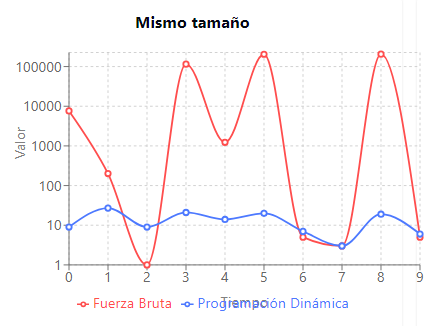
\includegraphics[width=\textwidth]{images/mismotamanio.png}
    \end{minipage}%
    \begin{minipage}[t]{0.5\textwidth}
        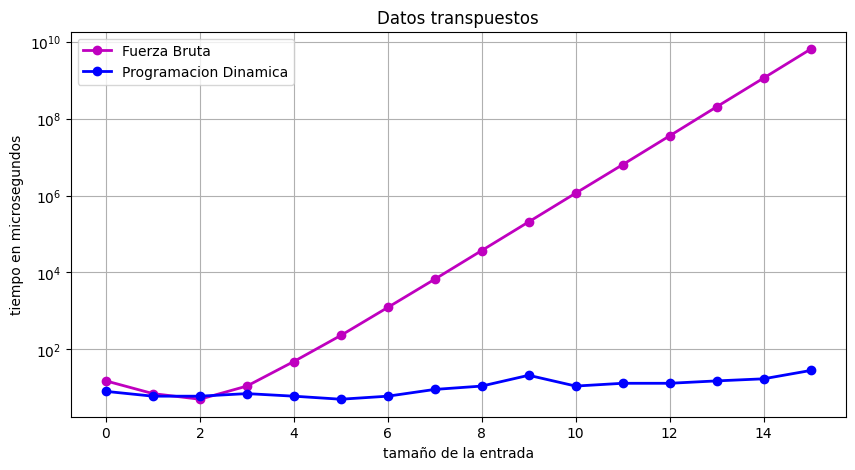
\includegraphics[width=\textwidth]{images/transpuesto.png}   \end{minipage}%
    \caption{Tiempos de ejecucion vs largo de las cadenas}
    \label{fig:Tiempos de ejecucion vs largo de las cadenas}
\end{figure}

\begin{figure}[H]
    \centering
    \begin{minipage}[t]{0.5\textwidth}
        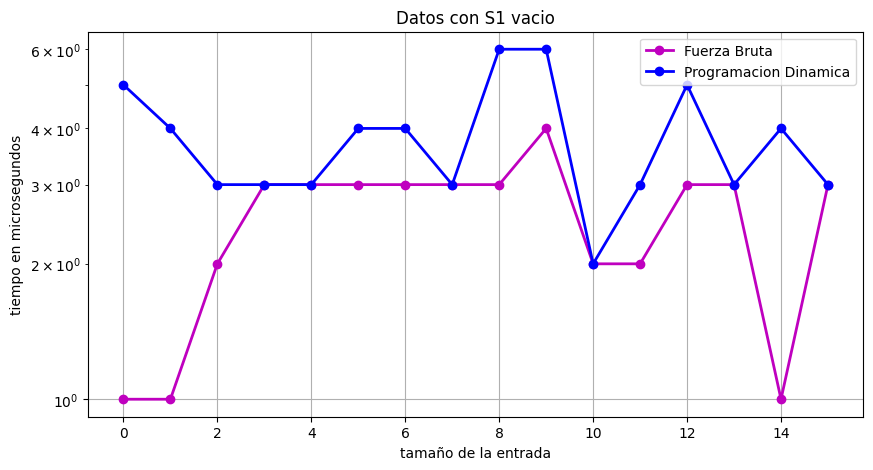
\includegraphics[width=\textwidth]{images/s1vacio.png}
    \end{minipage}%
    \begin{minipage}[t]{0.5\textwidth}
        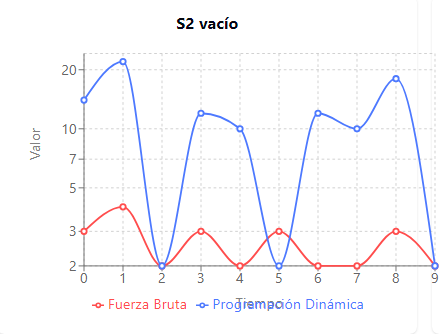
\includegraphics[width=\textwidth]{images/s2vacio.png}   \end{minipage}%
    \caption{Tiempos de ejecucion vs largo de las cadenas}
    \label{fig:Tiempos de ejecucion vs largo de las cadenas}
\end{figure}

\begin{figure}[H]
    \centering
    \begin{minipage}[t]{0.5\textwidth}
        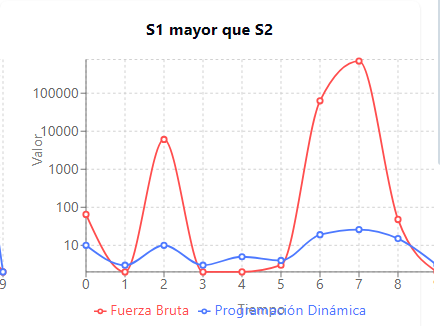
\includegraphics[width=\textwidth]{images/s1mayor.png}
    \end{minipage}%
    \begin{minipage}[t]{0.5\textwidth}
        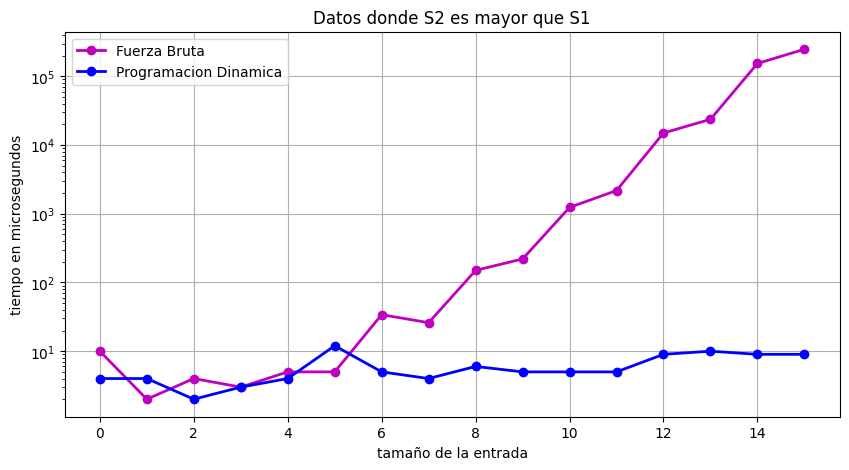
\includegraphics[width=\textwidth]{images/s1menor.png}   \end{minipage}%
    \caption{Tiempos de ejecucion vs largo de las cadenas}
    \label{fig:Tiempos de ejecucion vs largo de las cadenas}
\end{figure}
